\chapter{Analysis}
\label{chap:analysis}

Access to both spatially and spectrally resolved observations of protoplanetary disks offers a unique view into their chemical and physical characteristics, characteristics that we may discover through modeling. Modeling, in its essence, is the process of generating a synthetic image of what a disk with known physical characteristics (like disk radius, mass, and so on) would look like at a certain distance, inclination, and position angle relative to us. From that synthetic image, we may generate a synthetic set of visibilities, and then compare those visibilities to our observations. By iterating this process, we may generate many models with different parameter combinations and evaluate how well each resulting model disk matches our observations. Aggregating these results allows us to discover best-fit regions of parameter space, and thus make inferences about the nature of our sources based on those best-fit parameters.

% which regions of this parameter-space result in models which best match our data, and thus make inferences about the nature of our sources based on those best-fit parameters.

In \S\ref{section:gas_model}, we describe the basic equations and computational processes that generate the model disks. In \S\ref{section:param_space}, we describe how, once models are made, we may move through high-dimensional parameter space to identify regions of best-fit. Finally, in \S\ref{section:fitting_procedure}, we present the results of our fitting procedures.


\section{Gas Model}
\label{section:gas_model}

In this work, we use a gas-disk model originally developed by Rosenfeld et al. (2012a, 2013 reference) and translated from IDL to Python by Flaherty et al (2015 reference). The model begins by calculating the radial profiles for the disk in temperature, surface density, and velocity before performing radiative transfer on the resulting structure to create a sky-projected image of the model disk, taking into account line thermal and turbulent line broadening. The use of a few simplifying assumptions allows the code to run quickly enough to allow for a Markov Chain Monte Carlo routine to generate models on a reasonable timescale, as described in \S\ref{subsection:mcmc}



% We start with a temperature and surface density structure, compute the vertical structure using hydrostatic equilibrium, calculate the velocity field taking into account Keplerian rotation as well as pressure support, and compute the radiative transfer of the line through the disk, accounting for both thermal and turbulent broadening


\subsection{Establishing Physical Profiles}
A circumstellar disk can be characterized by three major profiles: its radial temperature structure, its radial density structure, and its velocity field. Generating a good model disk is a matter of defining these three functions appropriately.

However, these are complex functions, and the reality that they attempt approximate is an inherently wild, chaotic one; no disk's density actually falls off exponentially, although in some cases it can be well approximated as such. Furthermore, even these approximations often cannot be solved analytically, instead relying on numerical integration to be solved, which is a computationally expensive task. Therefore, we choose to make certain simplifying assumptions which, although they come at a cost to realism, enable significantly increased computation speeds.

The first major assumption that this code leverages is that the disk is under local thermal equilibrium (LTE). This assumption allows the use of a one-dimensional (radial) temperature profile, based on the assumption that local pockets of the disk are in equilibrium with one another and thus that the disk's temperature profile changes only with macroscopic causes, rather than local ones. While it is not clear whether the assumption of LTE is always a valid one in proplyds, it has been shown to be appropriate for CO (Pavlyuchenkov et al. (2007) reference). For this temperature profile, we draw on the parametrization of disk temperature structure first laid out by Dartois et al. (2003 reference), where the disk's temperature is given by,

\begin{align}
  T_{\text{gas}}(r, z) = \begin{cases}
                          T_a + (T_m - T_a) \left[ \cos \frac{\pi z}{2 z_q} \right]^{2\delta} \text{   if } z > z_q \\
                          T_a \text{   if } z \leq z_q(r).
                         \end{cases}
\end{align}

The atmospheric temperature and mid-plane temperatures are given by $T_a = T_{atm,150} (r/150 \text{AU})^{q}$ and $T_m = T_{mid, 150} (r/150 AU)^{q}$, where $q$ is typically negative and controls the functions' decay. Since $T_m$ is smaller than $T_a$, the second term of of the low-scale height temperature function is negative, so the sinusoid effectively implements a decreasingly-negative contribution to the temperature with hight above midplane.  The height of the disk, controlled by $z_q$ is assumed to be radially increasing, as described by a power law, $z_q(r) = z_{q,150}(r/150 \text{AU})^{1.3}$. This characteristic height controls how "puffy" the disk is, and consequently at what height we set the disk's atmosphere.

We set $\delta$ to 1, though it can take on values between 1-2 \textit{(what is $\delta$?)}.




The second primary assumption that this code makes is that the motions of the disks' gas are described by a Keplerian velocity field with no angular dependence. This assumption is valid in the case that $M_{\text{disk}} \ll M_{\star}$, which previous continuum observations of the disks have shown them to be. Slight modifications from a purely Keplerian profile are made to account for the pressure support of the gas and to add in a vertical dependence, yielding

\begin{align}
  \frac{v_\phi^2}{r} = \frac{GM_\star r}{(r + z)^{3/2}} + \frac{1}{\rho_\text{gas}} \frac{\partial P_\text{gas}}{\partial r};\,\, v_r = v_z = 0.
\end{align}


The third major assumption made is that the disk is under hydrostatic equilibrium. This assumption allows us to relate the disk's gas density and temperature profiles as

\begin{align}
  -\frac{\partial \ln \rho_\text{gas}}{\partial z} = \frac{\partial \ln T_\text{gas}}{\partial z} + \frac{1}{c_s^2} \left[\frac{G M_{\*} z}{(r^2 + z^2)^{3/2}} \right].
\end{align}

Here $c_s$ is the local sound speed, given by $c_s^2 = \frac{k_B T_\text{gas}}{\mu m_H}$, $T_\text{gas}$ is the temperature profile given above, $m_H$ the mass of hydrogen, and $\mu$ is the relative abundance of hydrogen in the disk, set here at 80\%. We may solve this equation by integration, giving us the disk's density profile $\rho(r, z)$.




The model's surface density is dscribed by a profile originally presented by Lynden-Bell & Pringle (1974 reference) and Hartmann et al. (1998 reference), in which they model a thin viscous accretion disk with a gas surface density profile given by

\begin{align}
  \Sigma_{\text{gas}}(r) = \frac{M_{\text{gas}} (2 - \gamma)}{2 \pi R_c^2} \left(\frac{r}{R_c} \right)^{-\gamma} \exp \left[-\left(\frac{r}{R_c} \right)^{2-\gamma} \right],
\end{align}

where $R_c$ is the radial extent of the gas disk, $\gamma$ is a power law index, and $M_\text{gas}$ is the total gas mass. This form allows the disk to increase radially as a power law until R$_c$, at which point it turns over into exponential decay. Exponentially tapering the disk's outer radius, rather than sharply cutting it, has been shown to be effective (Hughes et al (2008), Andrews et al (2010) reference). We may safely approximate $M_\text{gas} = M_\text{disk}$, since at this early stage in the disk's development, the gas is by far the majority element of the disk's mass total. \textit{Unclear to me what the relationship between $\rho(r, z)$ and $\Sigma(r)$ is - how do they relate?}

Modifications are made to this density profile in two cases. At sufficiently low temperatures, molecules will condense out of the gas phase. The mid-plane of the disk is sufficiently cold to prompt this behavior. We may simulate this behavior by dropping the gas density by a factor of $10^{-18}$ wherever the temperature falls below some characteristic freeze-out temperature, $T_{FO}$, a temperature which is molecule-specific. In this work, we use $T_{FO} = 19$K for HCO$^+$, CO, and CS, and $T_{FO} = 60$K for HCN (why is this again?). Conversely, at the disk's upper surface, photodissociation by stellar radiation dominates, so we implement a decrease in density wherever the hydrogen column density at the disk's surface falls below a characteristic value (for HCO$^+$, CO, and CS, this value is $1.3 \times 10^{-21} \text{cm}^{-2}$, whereas for HCN it is $9.5 \times 10^{-21} \text{cm}^{-2}$ (again, why, and also what's the other column density value that I feed into the model?)).



The resulting temperature and density structure of a typical proplyd is shown in Fig \ref{fig:temp_dens_str}.

\begin{figure}[htp]
\centering
  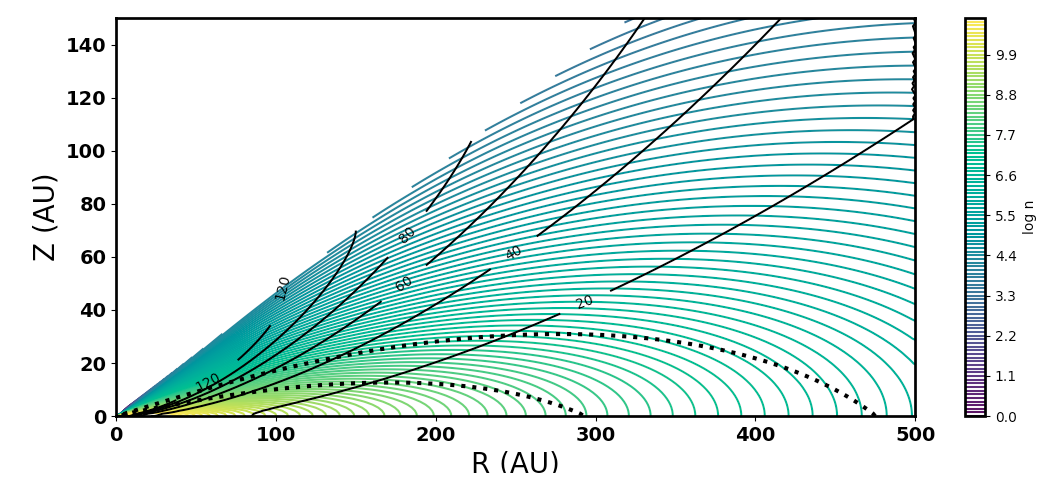
\includegraphics[width=\linewidth]{proplyd_temp_dens_str.png}
  \captionof{figure}{A disk structure plot.}
  \label{fig:temp_dens_str}
\end{figure}






\subsection{Generating a Model Image}

Having now established our model disk's physical structure through temperature, density, and velocity profiles, we may begin generating an image of the disk by calculating flux contributions through the disk. To do so, we calculate the specific intensity by integrating the equation of radiative transfer:

\begin{align}
  I_\nu = \int_0^{\infty} K_\nu(s)\ S_\nu(s)\ e^{-\tau_\nu(s)}\ ds,
\end{align}

where $K_\nu(s)$ is the absorption coefficient, $\tau_\nu(s)$ is the optical depth and is defined as $\tau_\nu(s) = \int_0^s K_\nu(s') ds'$, and $S_\nu(s)$ is the source function. Since disks emit as blackbodies, the Planck function, $B_\nu(T)$, is used as the source function. Line broadening, a function of temperature and disk turbulence, is added, and the resulting flux is Doppler shifted to account for the disk's specified systemic velocity. Finally, the image is scaled, shifted, and rotated to account for the source's distance ($d$), angular offset from the center of the image ($\Delta \alpha$ and $\Delta \delta$), and position angle and inclination (PA and $i$) relative to our viewing direction.


Since the model disk is fully defined at every point in both physical and velocity space, we may choose our spatial and spectral resolutions arbitrarily. We set our spectral resolution to match that of our observation, while we let the spatial resolution be $\sim$ 1/10 the size of the synthesized beam. This resolution is high enough to avoid sampling artifacts when we simulate interferometric observations of the image.

We then use the Miriad task \texttt{uvmodel} to generate visibilities from the model image, sampled in the same $uv$ tracks as our observation. The $\chi^2$ statistic is then used as a goodness-of-fit metric to compare the data and model in the visibility domain. We make this calculation in the visibility domain, rather than the image domain, so that the resulting $\chi^2$ value is not influenced by artifacts generated in the imaging process.



We now have the ability to generate a model disk, first by calculating its physical structures (in radial temperatures, densities, and velocities), then by drawing on radiative transfer to calculate the flux contributions from the disk. That flux is sky-projected to match the observed source's orientation, and the resulting image is then transformed from the image domain to the visibility domain and its fit quality evaluated. With this pipeline established, we now consider the various knobs we may turn to affect the resulting image. While there are many more adjustable parameters than those given below, these are the primary drivers of flux levels and thus the dimensions we fit for.

\begin{itemize}
  \item \textsc{Atmospheric Temperature} (T$_\text{atms, 150}$): The temperature at the disk's surface at 150 AU. Used as a scaling coefficient for the disk's radial temperature profile, as described above.
  \item \textsc{Outer Radius} (R$_c$): Effectively the outer radius of the gas disk, R$_c$ controls the turn-over point of the surface density profile, as described above. This can vary by line, thanks to different excitation temperatures, densities, and physical distributions of gas.
  \item \textsc{Radial Temperature Power Law Index} ($q$): The exponent of the power law that governs the disk's radial temperature structure, as described above.
  \item \textsc{Relative Molecular Abundance} ($X_\text{mol}$): The relative molecular abundance indicates the fractional abundance of the molecule under observation relative to the H$_2$ abundance. We fit for $X_\text{mol}$ for our HCO$^+$, HCN, and CS models, but fix it at the literature value of $10^{-4}$ for CO.
  \item \textsc{Log Disk Mass} ($\log M_{\text{disk}}$): The base-10 logarithm of each disk's mass. We fit for $\log M_{\text{disk}}$ only in the CO data, where $X_\text{mol}$ is fixed. In all other lines, it is left fixed.
  \item \textsc{Inclination} ($i$): The disk's inclination angle.
  \item \textsc{Position Angle} (PA): The disk's position angle.
\end{itemize}



A selection of the remaining parameters, which we leave fixed, are summarized in Table \ref{table:other_params}.

\centerline{Fixed Parameters \textbf{Not convinced that this is necessary. Incomplete at the moment.}}
\smallskip
\centerline{
%\begin{center}
  % \begin{tabular*}{\textwidth}{l@{\extracolsep{\fill}}c | l | l}
  \begin{tabular*}{\textwidth}{c | l | l}
    \hline \hline
    v$_{\text{sys}}$ & \textsc{Systemic velocity}  &  The line-of-sight velocity of the disk. \\ \hline
    $\Delta \delta, \Delta \alpha$ & \textsc{Position Offset}  & Each disk's distance from the center of the field of view. \\\hline
    M$_{\star}$ & \textsc{Stellar Mass}  &  The masses of each disk, from Someone et al (1900 reference). \\ \hline
    v$_{\text{sys}}$ & \textsc{Systemic velocity (km/s)}  &  The line-of-sight velocity of the disk. \\ \hline
    $d$ & \textsc{Distance}  &  The distance to the sources, from Gaia. \\
    \hline
    \caption{Some param values}
  \end{tabular*}
  \label{table:other_params}
}
%\end{center}



\section{Exploring Parameter Space}
\label{section:param_space}

Now that we have the tools available to generate synthetic images that are tuneable across a large number of parameters, we must decide how best to move through that large parameter space to find a best-fit region. To do so, we use two methods.

\subsection{Grid Search}
The first, and perhaps most intuitive, way to move through this parameter space is using a simple grid search. A grid search involves manually assembling lists of values to try for each parameter and then generating models and calculating the resulting $\chi^2$ value for every possible combination of parameters in those lists. A best-fit value is recovered by simply finding the point in that $n$-dimensional grid that yielded the best $\chi^2$, and then either calling that position in parameter space a best-fit location or then defining a finer grid around that point and repeating the process until an acceptable resolution has been reached. Benefits of grid search include its relatively straightforward nature (the the consequent simplicity of implementation) and its usefullness as a diagnostic tool, since very specific regions of parameter space may be sampled with the manual entry of positions to test. However, it is a relatively simple method and leaves room for improvement.


\subsection{Markov Chain Monte Carlo}
\label{subsection:mcmc}

Markov Chain Monte Carlo (MCMC) algorithms offer us a way to both sample the probability distribution of a complex parameter space (much like a grid search), but offer an improvement over grid search by yielding the posterior probability distribution of each point, allowing us to characterize the uncertainty associated with each best-fit value with error bars. We use an affine-invariant formulation of the MCMC algorithm described by Goodman \& Weare (2010 reference) and implemented in the Python package \textittt{emcee} by Foreman-Mackey et al 2013 (reference).

MCMC routines sample the probability distribution of a given $n$-dimensional parameter space by deploying an army of "walkers." Each walker begins at some initial position, evaluates the $\chi^2$ value of that point, and then proposes moving to a new position in parameter space according to a Gaussian probability distribution centered at the current point and decaying with distance (so that nearer points are preferentially - but not necessarily - selected). The $\chi^2$ value of this new position - or "step" - is then evaluated, and is either accepted (the walker moves to that position) or rejected (the walker remains where it is and repeats the new-step proposal process) with probability $p = \exp \left[ (\chi_\text{current}^2 - \chi_\text{new}^2)/2 \right]$ (is this only for Metropolis Hastings?). This function indicates that if the proposed step yields a better fit (a lower $\chi^2$ value) than the current position, $p > 1$ and the step is accepted. However, if proposed step results in a worse fit, there is still a non-zero chance that the step is accepted, proportional to how much worse it is. This willingness to accept an increased $\chi^2$ value allows the walker to avoid becoming trapped in local minima. The list of steps taken by each walker and their accompanying $\chi^2$ values are compiled into the "chain" part of Markov Chain Monte Carlo. It has been demonstrated (reference?) that a walker's desire to remain in a location is proportional to the local probability density, meaning that we may infer uncertainties in our fits from the density of walker steps taken in a region.

We may introduce boundaries to the parameter space explored by our walkers using "priors." These priors are manually set, and allow us to save time by restricting the walkers' motions into regions that we know a priori to be implausible fits. The priors used for this project are given in Table \ref{table:priors}.

\bigskip
\centerline{Priors for Fit Parameters \textbf{Probably have to make this long format.}}
\smallskip
\centerline{
% \begin{tabular*} {c | c | c | c | c | c}
\begin{tabular*}{\textwidth}{l@{\extracolsep{\fill}}c | c | c | c | c | c}
  \hline \hline
  Disk                & R$_{\text{out}}$  & T$_\text{atms}$ & $i$     & PA       & X$_\text{mol}$  & \log M$_\text{disk}$ & Tqq     \\ \hline
  \textbf{A} & (10, 1000)        & (0, 1000)       & (0, 90) & (0, 360) & (-13, -3)       & (-2.5, 0)            & (-3, 3) \\
  \textbf{B} & (10, 1000)        & (0, 1000)       & (0, 90) & (0, 360) & (-13, -3)       & Fixed                & Fixed   \\
  \hline
  \caption{Some param values}
\end{tabular*}
}
\label{table:priors}

We may visualize our results using corner plots. Corner plots allow high-dimensional space to be visualized in two dimensions by taking slices across each pair of axes and showing the density of samples drawn in that slice. In each of these slices, a perfectly certain fit would appear as a very tight Gaussian - the sample density around the best fit would be extremely high and low everywhere else - while conversely, higher uncertainties are shown by a wide spread of samples around the central point. Degeneracies between parameters can be seen in non-point-like distributions of samples (i.e. some correlation between dimensions). Corner plots for Disk A and B in an HCO$^+$ fit are shown in Figs \ref{fig:corner_a} and \ref{fig:corner_b}, respectively.


\begin{figure}[htp]
  % Maximum length
  % \subcaptionbox{1a\label{fig1:a}}{\includegraphics[width=1.6in]{example-image-a}}\hfill%
  % \subcaptionbox{1b\label{fig1:b}}{\includegraphics[width=1.6in]{example-image-a}}%
  % \bigskip
  % Equal length
  \hspace*{\fill}%
  \subcaptionbox{Disk A fits \label{fig:corner_a}}{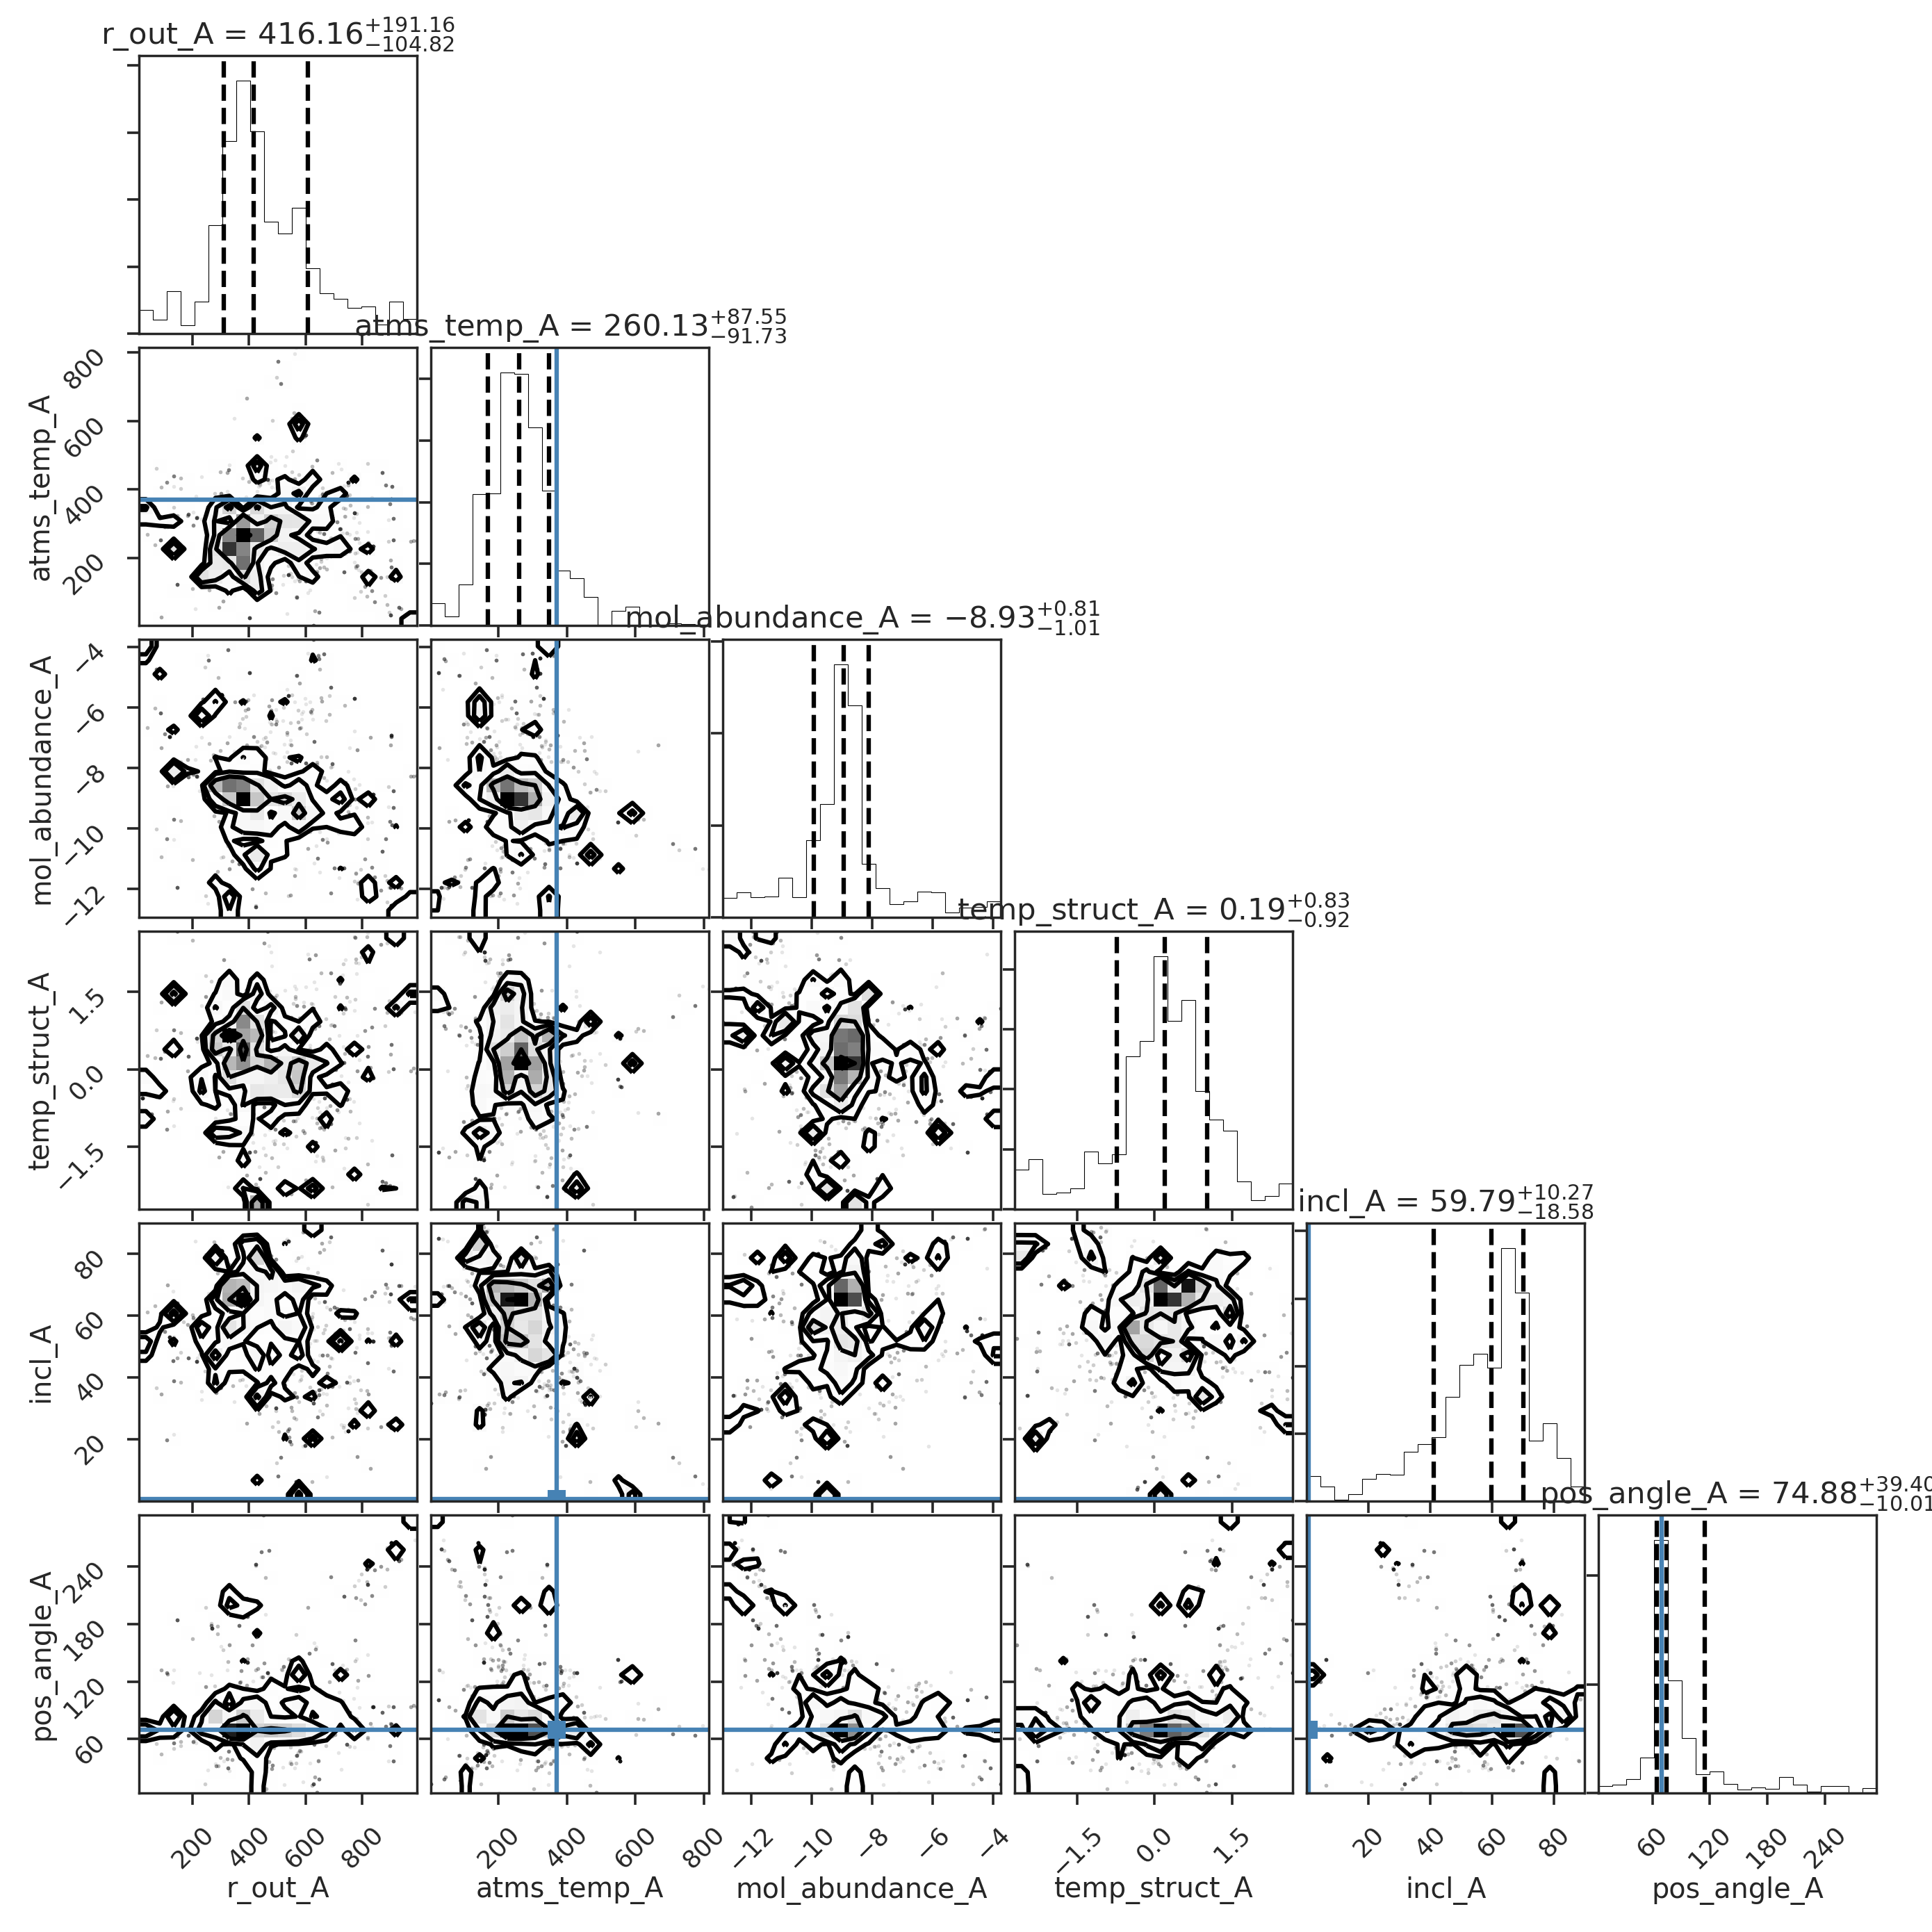
\includegraphics[width=0.48\linewidth]{cornerplot-diskA.png}}\hfill%
  \subcaptionbox{Disk B fits \label{fig:corner_b}}{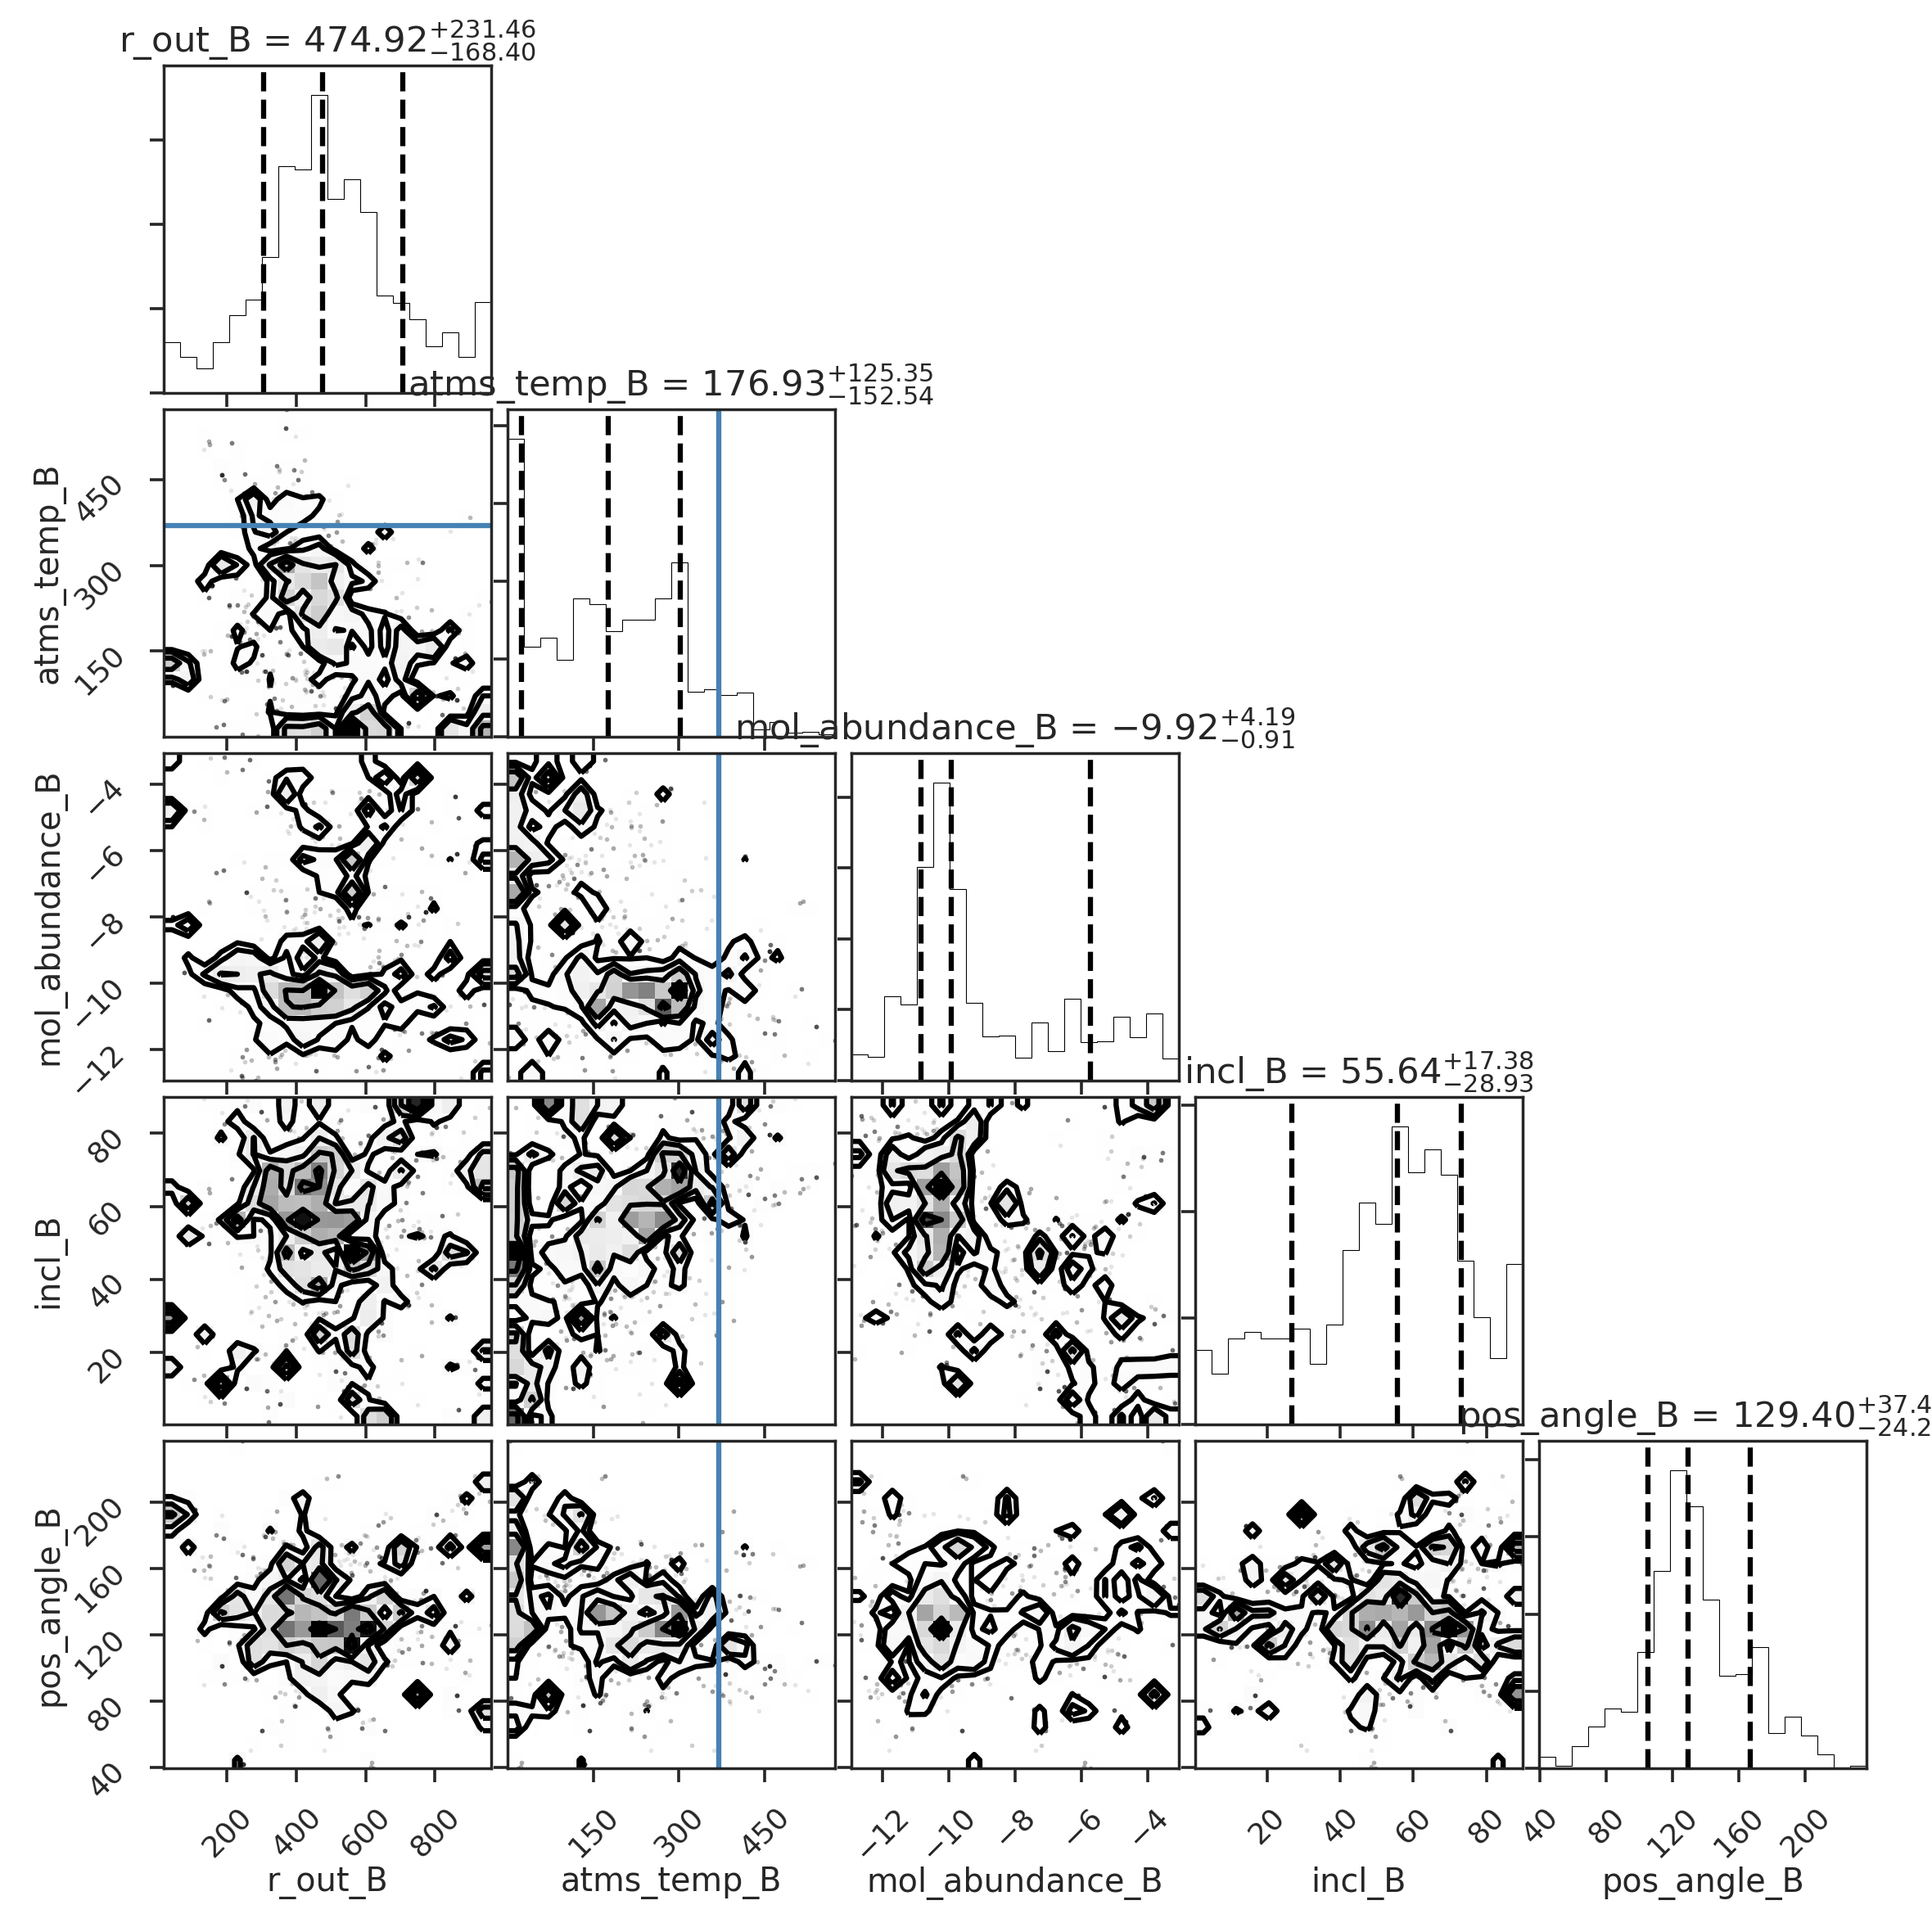
\includegraphics[width=0.48\linewidth]{cornerplot-diskB.png}}%
  \hspace*{\fill}%
  \caption{This probably isn't the place for these, but just wanted to make sure they were working. They might also be a little small when they're side by side like this.}
  \label{fig:corner_plots}
\end{figure}





\section{Fitting Procedure}
\label{section:fitting_procedure}

Fitting of the data began with the analysis and partial removal of cloud contamination discussed in Section \ref{section:cloud_contamination}, resulting in the removal of baselines below a characteristic length for each line. With the data as clean as possible, position ($\alpha, \delta$) and velocity ($v_\text{sys}$) offsets were fit for. To do so, all disk parameters were fixed at hand-selected, ballpark-reasonable values and ran a grid search over RA/dec offsets and systemic velocities for each disk, using grid resolutions that corresponded to the beam width and spectral resolution, respectively. Offset fitting was executed only in the HCO$^+$ line, thanks to the line's minimal contamination and high signal. Positional offsets were confirmed with elliptical Gaussians in \texttt{CASA}. The results of this procedure are reported in Table \ref{table:offsets}.

\bigskip
\centerline{XYV Offsets }
\smallskip
\centerline{
% \begin{tabular*} {c | c | c | c | c | c}
\begin{tabular*}{\textwidth}{l@{\extracolsep{\fill}}c | c | c | c }
  \hline \hline
                  & \textbf{$\alpha$}  & \textbf{$\delta$} & $v$ \\ \hline
  \textbf{Disk A} & 0.0002             & 0.082             & 10.0 \\
  \textbf{Disk B} & -1.006             & -0.3              & 10.75 \\
  \hline
  \caption{OffsetsLooking bad now, will get better later}
\end{tabular*}
}
\label{table:offsets}





\bigskip \bigskip \bigskip
Should probably put uncertainties into these reports. Also probably don't need a subsection for every line, just the important ones. Will depend on results.


\subsection{CO (3-2) Fit}
Starting with CO to get disk mass.

Best fit values are reported in Table \ref{table:bf_co}

\bigskip
\centerline{CO (3-2) Best-Fit Paramers}
\smallskip
\centerline{
% \begin{tabular*} {c | c | c | c | c | c}
\begin{tabular*}{\textwidth}{l@{\extracolsep{\fill}}c | c | c | c | c | c}
  \hline \hline
         & R$_{\text{out}}$  & T$_\text{atms}$ & $i$     & PA  & \log M$_\text{disk}$ & Tqq \\ \hline
  Disk A & 1                 & 1               & 1       & 1   & 1                    & 1   \\
  Disk B & 1                 & 1               & 1       & 1   & 1                    & 1   \\
  \hline
  \caption{Some best-fit CO param values}
\end{tabular*}
}
\label{table:bf_co}




\subsection{HCO$^+$ (4-3) Fit}
Then the rest of them, probably HCO next because low contamination.

Best fit values are reported in Table \ref{table:bf_hco}

\bigskip
\centerline{HCO$^+$ (4-3) Best-Fit Paramers}
\smallskip
\centerline{
% \begin{tabular*} {c | c | c | c | c | c}
\begin{tabular*}{\textwidth}{l@{\extracolsep{\fill}}c | c | c | c | c | c}
  \hline \hline
         & R$_{\text{out}}$  & T$_\text{atms}$ & $i$     & PA  & \log M$_\text{disk}$ & Tqq \\ \hline
  Disk A & 1                 & 1               & 1       & 1   & 1                    & 1   \\
  Disk B & 1                 & 1               & 1       & 1   & 1                    & 1   \\
  \hline
  \caption{Some best-fit HCO+ param values}
\end{tabular*}
}
\label{table:bf_hco}




\subsection{HCO$^+$ (4-3) Fit}
Then the rest of them, probably HCO next because low contamination.

Best fit values are reported in Table \ref{table:bf_hcn}

\bigskip
\centerline{HCN (4-3) Best-Fit Paramers}
\smallskip
\centerline{
% \begin{tabular*} {c | c | c | c | c | c}
\begin{tabular*}{\textwidth}{l@{\extracolsep{\fill}}c | c | c | c | c | c}
  \hline \hline
         & R$_{\text{out}}$  & T$_\text{atms}$ & $i$     & PA  & \log M$_\text{disk}$ & Tqq \\ \hline
  Disk A & 1                 & 1               & 1       & 1   & 1                    & 1   \\
  Disk B & 1                 & 1               & 1       & 1   & 1                    & 1   \\
  \hline
  \caption{Some best-fit HCN param values}
\end{tabular*}
}
\label{table:bf_hcn}





\subsection{CS (7-6) Fit}
Blah blah blah
Best fit values are reported in Table \ref{table:bf_cs}

\bigskip
\centerline{CS (7-6) Best-Fit Paramers}
\smallskip
\centerline{
% \begin{tabular*} {c | c | c | c | c | c}
\begin{tabular*}{\textwidth}{l@{\extracolsep{\fill}}c | c | c | c | c | c}
  \hline \hline
         & R$_{\text{out}}$  & T$_\text{atms}$ & $i$     & PA  & \log M$_\text{disk}$ & Tqq \\ \hline
  Disk A & 1                 & 1               & 1       & 1   & 1                    & 1   \\
  Disk B & 1                 & 1               & 1       & 1   & 1                    & 1   \\
  \hline
  \caption{Some best-fit CS param values}
\end{tabular*}
}
\label{table:bf_cs}






% The End
